\documentclass[ignorenonframetext]{beamer} 
%\documentclass{article}
%\usepackage{beamerarticle}

\usepackage{beamerthemesplit}
\usepackage{color}

\usepackage{amsmath,amssymb,amsthm}
\hypersetup{unicode=true}
\DeclareFontEncoding{T1}
\fontencoding{T1}
\usepackage[T2A]{fontenc}
\usepackage[utf8]{inputenc}
\usepackage[russian]{babel}
\usepackage{graphics,graphicx}
\usepackage{indentfirst}

\usepackage{verbatim}
\usepackage{fancyvrb}

\definecolor{codecolor}{RGB}{0,0,100}
\newcommand{\matcode}[1]{ \textcolor{codecolor}{\texttt{#1}}}

%\newcommand{\matcode}[1]{\begin{Verbatim}[formatcom=\color{red}]#1\end{Verbatim}}

\usetheme{CambridgeUS}
\usecolortheme{lily}


\title{Основы MATLAB}
\subtitle{Лекция 3. Высокоуровневая графика}
\author{Кафедра Т. М.}
\small
\institute[СГАУ]
{
Самарский государственный аэрокосмический университет им. академика С.~П.~Королёва \\
(национальный исследовательский университет)\\
\medskip
{\emph{yudintsev@termech.ru}}
}
\date{}

\begin{document}

\frame{\titlepage}

\frame{\tableofcontents}

\frame
{
  \frametitle{Два типа графики}
  Типы файлов: 
  \begin{itemize}
    \item \emph{высокоуровневая графика} \\
    минимум усилий пользователя: 
    автоматически выбираются свойства графиков (масштаб, цвет, шрифт, ...)
    \item \emph{интерактивная графика} \\	
    \item \emph{дескрипторная графика} \\
    пользователь сам определяет свойства графиков в тексте программы
  \end{itemize}
}

\section{Функции одной переменной}

\frame[containsverbatim]
{
  \frametitle{Построение графиков в окне Workspace}
  \begin{itemize}
   \item создать массив x: \matcode{x=0:0.1:10;} 
   \item создать массив y: \matcode{y=sin(x);}
   \item В окне \textbf{Workspace} выбрать переменные x и y (удерживая \texttt{[Ctrl]}) и по правой кн. мыши выбрать в контекстном меню \matcode{plot(x,y)}.
  \end{itemize}
}

\frame[containsverbatim]
{
  \frametitle{Типы графиков}
  В контектсном меню можно открыть каталог типов графиков
  \begin{figure}[h]
  \centering
  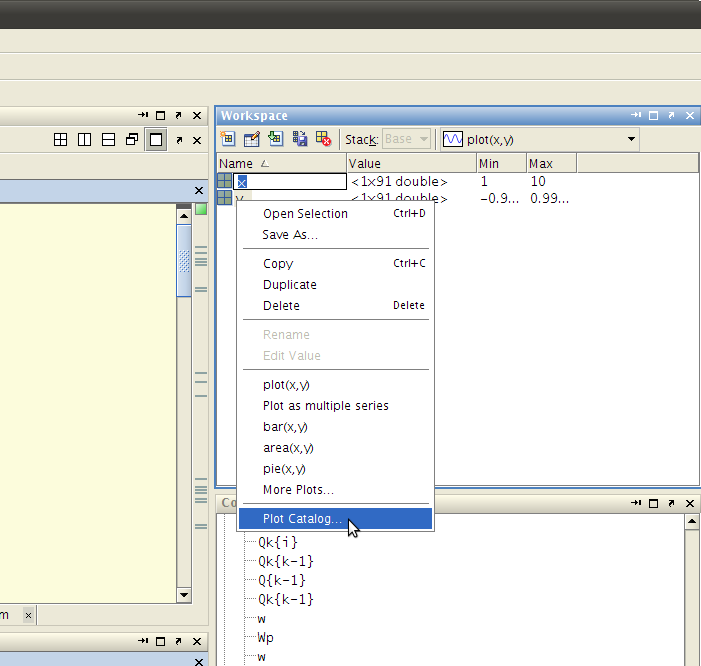
\includegraphics[width=0.6\linewidth]{./Screenshot-MATLAB_Worspace_plot.png}
  \end{figure}
}
\frame[containsverbatim]
{
  \frametitle{Типы графиков}
\begin{figure}[h]
 \centering
 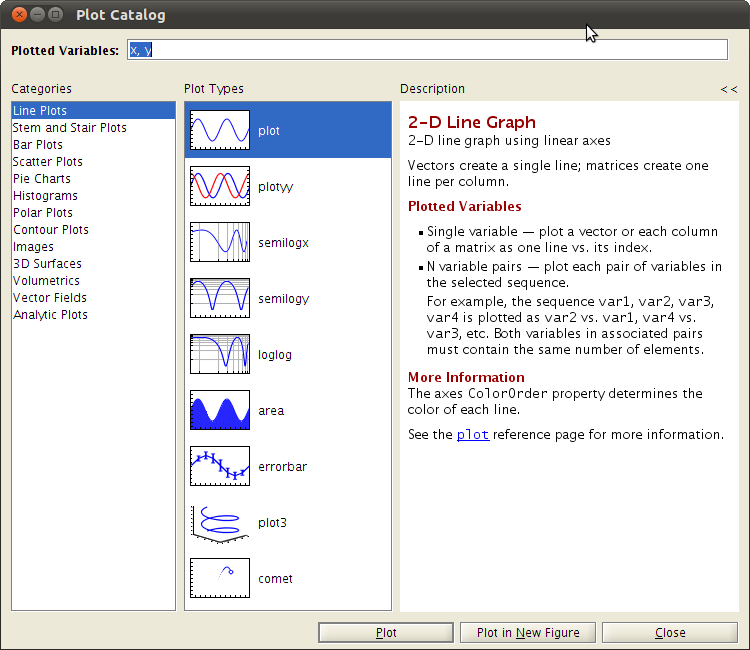
\includegraphics[width=0.6\linewidth]{./Screenshot-Plot_Catalog.png}
 % Screenshot-Plot Catalog.png: 750x650 pixel, 72dpi, 26.46x22.93 cm, bb=0 0 750 650
\end{figure}
}


\frame[containsverbatim]
{
  \frametitle{Функция fplot}
  \matcode{fplot('f(x)', [xmin xmax])}
}


\frame[containsverbatim]
{
  \frametitle{Функция plot}
  \begin{Verbatim}[formatcom=\color{codecolor}]
  x=0:0.1:5;
  plot(x,sin(x))
  \end{Verbatim}
}


\frame[containsverbatim]
{
  \frametitle{Построение графика из Command window и из Workspace window}
  \begin{itemize}
   \item plot(x,y)
   \item plot(x,y,'style')
  \end{itemize}
  'style' - строка, задающая цвет, тип маркера и тип линии. \\
  \matcode{(y,m,c,r,g,b,w,k)} -- цвет \\
  \begin{Verbatim}
(. x * + s d v ^ < > p h)}
  \end{Verbatim} -- тип маркера \\
  \matcode{(- : -. --)} -- тип линии
}


%
% Графики в логарифмических масштабах
%
\frame[containsverbatim]
{
  \frametitle{Гистограммы}
  \begin{itemize}
   \item \matcode{loglog} - логарифмический масштаб по обеим осям.
   \item \matcode{semilogx} - логарифмический масштаб по оси абсцисс.
   \item \matcode{semilogy} - логарифмический масштаб по оси ординат.   
  \end{itemize}
  \begin{Verbatim}[formatcom=\color{codecolor}]
  x=0.1:0.01:10;    
  y=log(0.5*x);
  g=sin(log(x));
  semilogx(x,y,x,g);
  \end{Verbatim}
}


\frame[containsverbatim]
{
  \frametitle{Столбчатые диаграммы}
\begin{columns}
\column{.4\textwidth}  
\begin{itemize}
   \item \matcode{x=1:0.2:3;}
   \item \matcode{y=sin(x);}
   \item \matcode{bar(y);} 
   \item \matcode{bar(x,y);}
   \item 3D версии - \matcode{bar3(x), bar3(x,y)}
\end{itemize}
\column{.6\textwidth}  
\begin{center}
 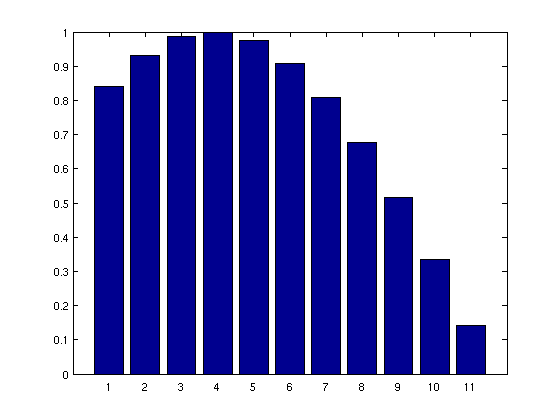
\includegraphics[width=1\linewidth]{./bar.png}
 % bar.png: 560x420 pixel, 90dpi, 15.81x11.85 cm, bb=0 0 448 336
\end{center}
\end{columns}
}

\frame[containsverbatim]
{
\frametitle{Круговые диаграммы}
\begin{columns}
\column{.5\textwidth}
  \begin{itemize}
   \item \matcode{x=[1,2,3,4];}
   \item \matcode{y=[0,0,1,0];}
   \item \matcode{pie(x)} -- показывает вклад кажого элемента вектора x в общую сумму.
   \item \matcode{pie(x,y)} -- логический массив (1,0), указывающий на необходимость изображение соответствующего сектора отдельно от круговой диаграммы.
  \end{itemize}
\column{.5\textwidth}
\begin{center}
 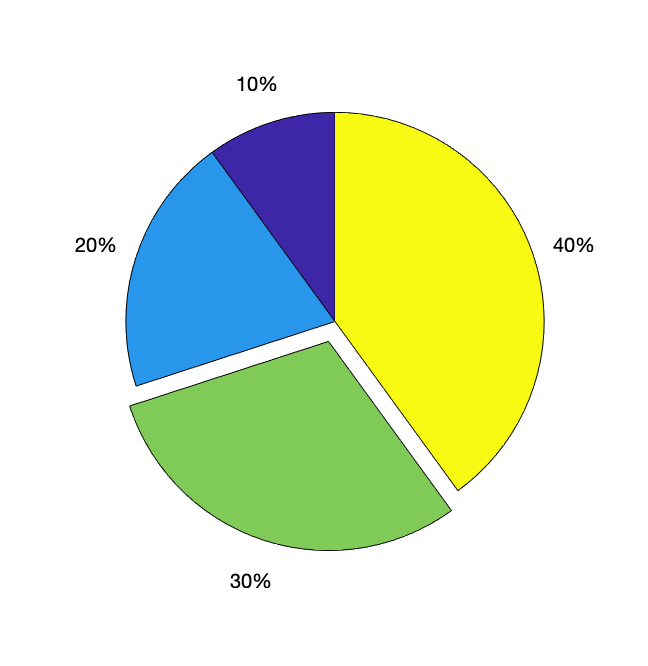
\includegraphics[width=1\linewidth]{./pie.png}
\end{center}  
\end{columns}
}

\frame[containsverbatim]
{
\frametitle{Круговые диаграммы}
Если сумма элементов массива данных больше или равна единице, то эта сумма принимается за 100\%, в противном случае строится диаграмма с пропущенным сектором.
\begin{columns}
\column{.5\textwidth}
  \begin{itemize}
   \item \matcode{x=[0.1,0.2,0.5];}
   \item \matcode{sum(x)} \\
\matcode{ans =} \\
\matcode{0.8000}
   \item \matcode{pie(x)}
  \end{itemize}
\column{.5\textwidth}
\begin{center}
 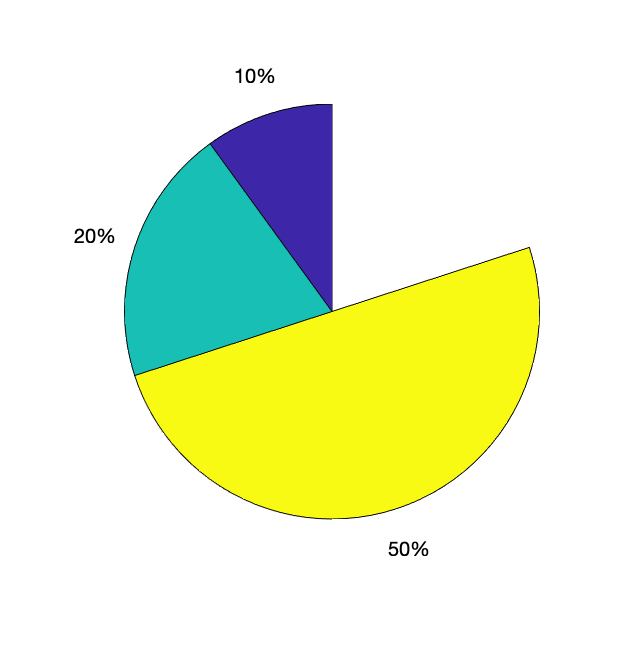
\includegraphics[width=1\linewidth]{./pie-sec.png}
\end{center}  
\end{columns}
}


\frame[containsverbatim]
{
  \frametitle{Гистограммы}
\begin{columns}
\column{.5\textwidth}
  \begin{itemize}
   \item Вектор-строка 100 случайных чисел, распределённых по нормальному закону с $m=0$ и $\sigma = 2$ \matcode{y=random('norm',0,2,1,100);}
   \item Функция \matcode{hist(y)} делит интервал y  на 10 частей и строит гистограмму.
  \end{itemize}
\column{.5\textwidth}
\begin{center}
 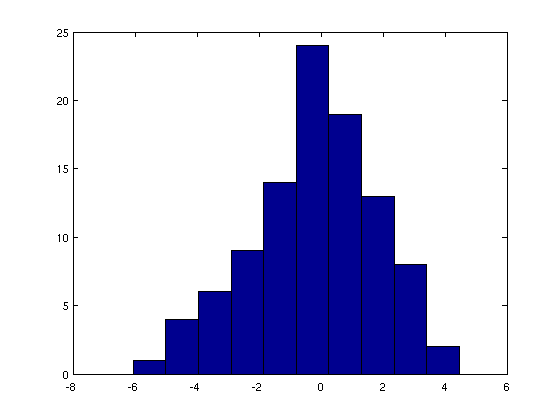
\includegraphics[width=1\linewidth]{./hist.png}
\end{center}  
\end{columns}
}


\frame[containsverbatim]
{
  \frametitle{Гистограммы}
\begin{columns}
\column{.5\textwidth}
  \begin{itemize}
   \item \matcode{hist(data,centers)} - вектор \matcode{centers} содержит центры интервалов 
   \item \matcode{hist(y,-6:1:6);}
   \item \matcode{histc(y,edges);} - вектор \matcode{edges} задаёт границы интервалов (монотонно возрастающая последовательность) 
   \item 3D версии - \matcode{bar3(x), bar3(x,y)}
  \end{itemize}
\column{.5\textwidth}
\begin{center}
 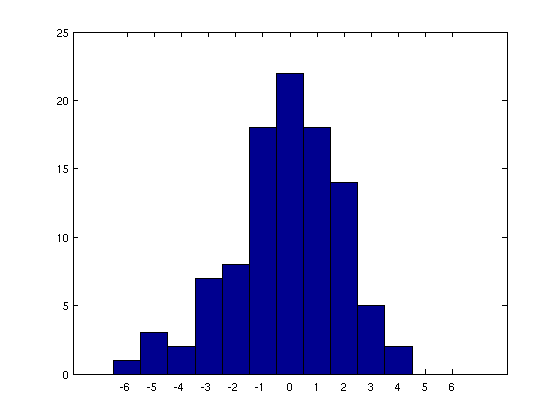
\includegraphics[width=1\linewidth]{./hist_centers.png}
\end{center}  
\end{columns}
}

\frame[containsverbatim]
{
  \frametitle{Круговая гистограмма}
\begin{columns}
\column{.5\textwidth}
  \begin{itemize}
   \item Генерируем вектор-строку 100 случайных чисел, распределённых по нормальному закону с $m=0$ и $\sigma = 1$ \matcode{y=random('norm',0,1,1,100);}
   \item \matcode{rose(y)} - строит гистограмму в полярных координатах, предполагая, что элементы массива \matcode{y} заданы в радианах.
  \end{itemize}
\column{.5\textwidth}
\begin{center}
 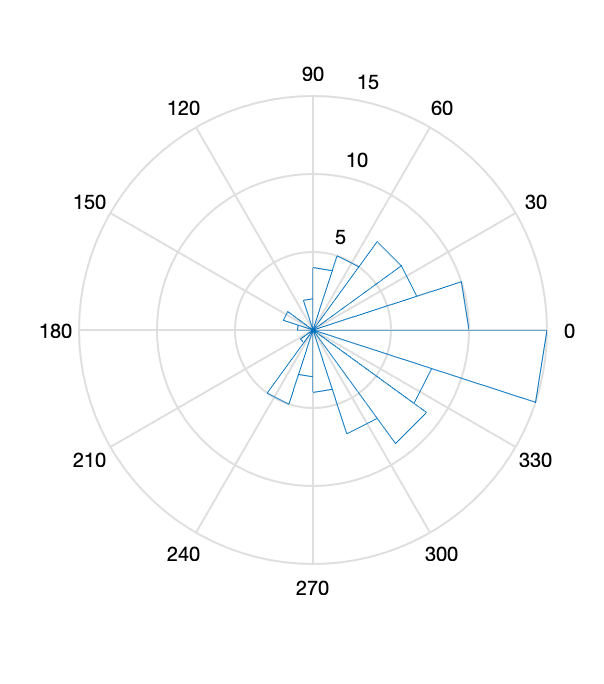
\includegraphics[width=1\linewidth]{./rose.png}
\end{center}  
\end{columns}
}

\section{Функции двух переменных}

\frame[containsverbatim]
{
\frametitle{Сетки и поверхности}
\begin{columns}
\column{.5\textwidth}
  \begin{itemize}
   \item генерация сетки \matcode{[X,Y]=meshgrid(-1:0.1:1,-1:0.1:1);}
   \item \matcode{Z=X.\textasciicircum2+Y.\textasciicircum2;}
   \item построение графика \matcode{mesh(X,Y,Z);}
   \item построение графика \matcode{surf(X,Y,Z);}
   \item \matcode{colorbar;} - добавить цветовой масштаб.
   \item \matcode{surf(X,Y,Z);} - поверхность с линиями уровня на плоскости (x,y).
  \end{itemize}
\column{.5\textwidth}
\begin{figure}[t]
 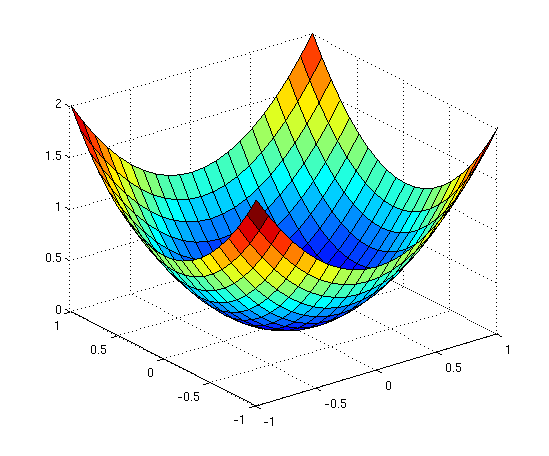
\includegraphics[width=6cm]{./surf.png}
 % contourplot.pdf: 612x792 pixel, 72dpi, 21.59x27.94 cm, bb=0 0 612 792
\end{figure}
\end{columns}
}


\frame[containsverbatim]
{
\frametitle{Контурные графики}
\begin{columns}
\column{.5\textwidth}
 \begin{itemize}
   \item \matcode{[X,Y]=meshgrid(-1:0.1:1,...}
   \matcode{-1:0.1:1);}
   \item \matcode{Z=X.\textasciicircum2+Y.\textasciicircum2;}
   \item \matcode{contour(X,Y,Z);} 
   \item \matcode{[c,h]=contour(X,Y,Z));} 
   \item \matcode{clabel(c,h);} 
   \item \matcode{grid on;}
 \end{itemize}
\column{.5\textwidth}
\begin{figure}[t]
 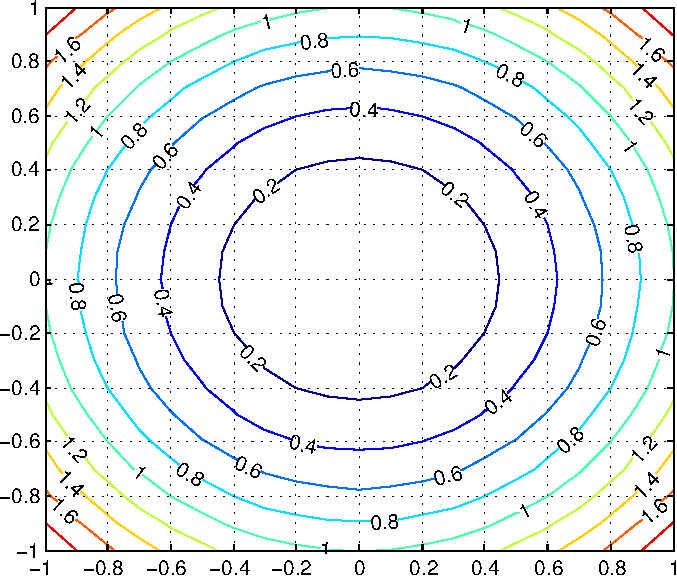
\includegraphics[width=5cm]{./contourplot.pdf}
 % contourplot.pdf: 612x792 pixel, 72dpi, 21.59x27.94 cm, bb=0 0 612 792
\end{figure}
\end{columns}
}

\frame[containsverbatim]
{
\frametitle{Контурный график с заливкой}
\begin{columns}
\column{.5\textwidth}
 \begin{itemize}
   \item \matcode{contourf(X,Y,Z,10);} 
   \item \matcode{colorbar;}
 \end{itemize}
\column{.5\textwidth}
\begin{figure}[t]
 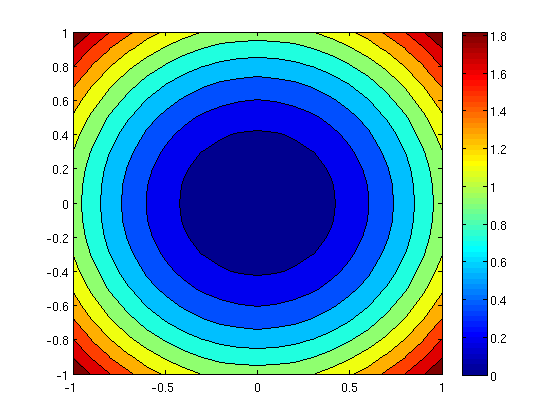
\includegraphics[width=5.5cm]{./contourf.png}
 % contourplot.pdf: 612x792 pixel, 72dpi, 21.59x27.94 cm, bb=0 0 612 792
\end{figure}
\end{columns}
}

\frame[containsverbatim]
{
\frametitle{Палитра графиков с цветовой заливкой}
\begin{columns}
\column{.5\textwidth}
 \begin{itemize}
   \item \matcode{contourf(X,Y,Z,10);} 
   \item \matcode{colorbar;}
   \item \fbox{\matcode{colormap(gray);}}    
 \end{itemize}
\column{.5\textwidth}
\begin{figure}[t]
 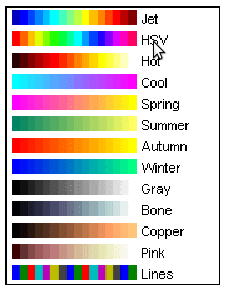
\includegraphics[width=4cm]{./colormap.png}
 % contourplot.pdf: 612x792 pixel, 72dpi, 21.59x27.94 cm, bb=0 0 612 792
\end{figure}
\end{columns}
}

\frame[containsverbatim]
{
\frametitle{Подписи к графикам в формате TeX}
\begin{columns}
\column{.5\textwidth}
\begin{itemize}
   \item \matcode{contourf(X,Y,Z,10);} 
   \item \matcode{colorbar;}
   \item \matcode{colormap(gray);}    
   \item \fbox{\matcode{title('z=x\textasciicircum2+y\textasciicircum2');}}    
 \end{itemize}
\column{.5\textwidth}
\begin{figure}[t]
 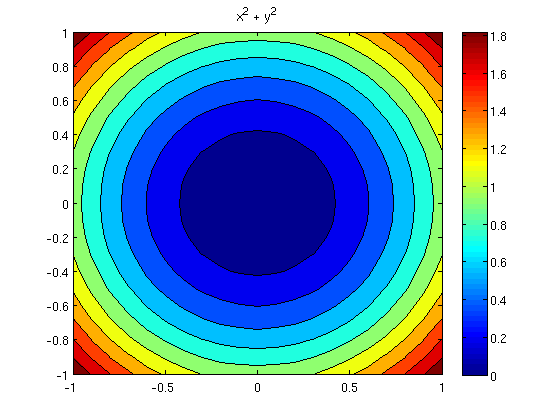
\includegraphics[width=6cm]{./contourf-tex.png}
 % contourplot.pdf: 612x792 pixel, 72dpi, 21.59x27.94 cm, bb=0 0 612 792
\end{figure}
\end{columns}
}


\frame[containsverbatim]
{
\frametitle{Параметрические кривые в пространстве}
\begin{columns}
\column{.5\textwidth}
\begin{itemize}
   \item \matcode{t=0:0.1:20;} 
   \item \matcode{x=cos(t);}
   \item \matcode{y=sin(t);}    
   \item \matcode{z=t;}    
   \item \matcode{plot3d(x,y,z);}    
 \end{itemize}
\column{.5\textwidth}
\begin{figure}[t]
 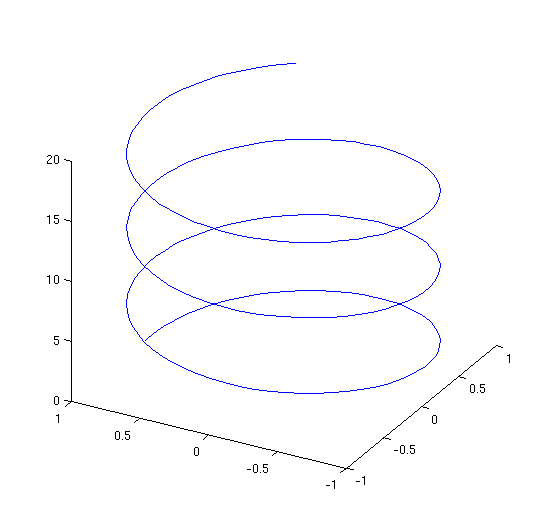
\includegraphics[width=6cm]{./plot3d.png}
 % contourplot.pdf: 612x792 pixel, 72dpi, 21.59x27.94 cm, bb=0 0 612 792
\end{figure}
\end{columns}
}

\frame[containsverbatim]
{
\frametitle{Поворот пространственного графика}
\begin{columns}
\column{.5\textwidth}
\begin{itemize}
   \item \matcode{view(az,el);} - задать новое положение наблюдателя.
   \item \matcode{[Az,El]=view;} - определить положение наблюдателя.
   \item \matcode{view(0,0);} - взгляд направлен вдоль оси y.    
 \end{itemize}
\column{.5\textwidth}
\begin{figure}[t]
 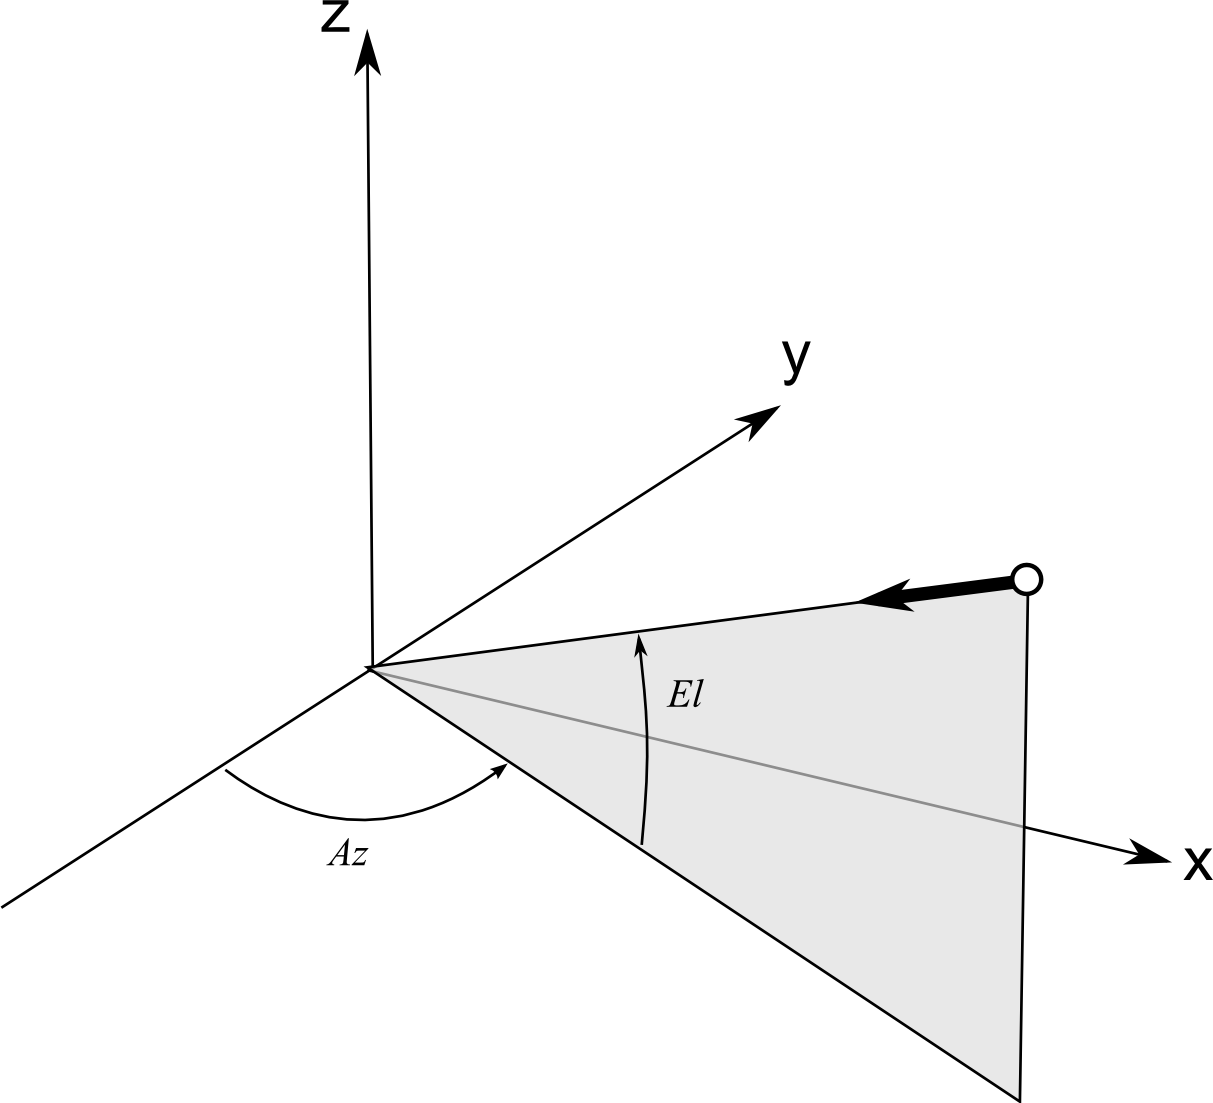
\includegraphics[width=5.5cm]{./AzEl.png}
 % contourplot.pdf: 612x792 pixel, 72dpi, 21.59x27.94 cm, bb=0 0 612 792
\end{figure}
\end{columns}
}

\frame[containsverbatim]
{
\frametitle{Освещенная поверхность}
\begin{columns}
\column{.5\textwidth}
\begin{itemize}
   \item \matcode{surfl(X,Y,Z,[Az,El]);} - отобразить поверхность с заданным азимутом и возвышением источника света.
   \item \matcode{colormap('copper');} - палитра copper.
   \item \matcode{shading interp;} - сглаживать цвета.    
 \end{itemize}
\column{.5\textwidth}
\begin{figure}[t]
 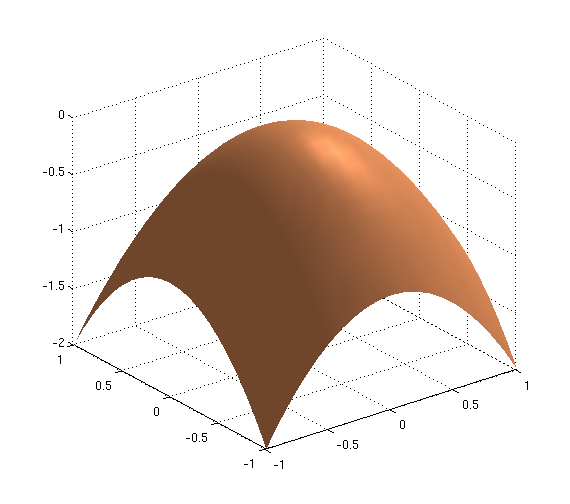
\includegraphics[width=5.5cm]{./surfl.png}
 % contourplot.pdf: 612x792 pixel, 72dpi, 21.59x27.94 cm, bb=0 0 612 792
\end{figure}
\end{columns}
}


\frame[containsverbatim]
{
\frametitle{Анимированные графики. Функция comet.}
  На плоскости:
  \begin{itemize}
   \item \matcode{t=0:0.01:10;}
   \item \matcode{x=t-sin(t);}
   \item \matcode{y=1-cos(t);}
   \item \matcode{comet(x,y);} или \matcode{comet(x,y,tail\_length);} \matcode{tail\_length} $\in (0\ldots1)$.
  \end{itemize}
  В пространстве:
  \begin{itemize}
   \item \matcode{t=0:0.01:10;}
   \item \matcode{x=cos(t);}
   \item \matcode{y=sin(t);}
   \item \matcode{z=t;}
   \item \matcode{comet3(x,y,z);} или \matcode{comet3(x,y,z,tail\_length);}
  \end{itemize}
}

\section{Форматирование графиков}

\frame[containsverbatim]
{
  \frametitle{Подписи к осям}
  \begin{Verbatim}[formatcom=\color{codecolor}]
plot(x,y1,x,y2);
grid on;
title('Скорости точек 1 и 2');
xlabel('t, c');
xlabel('v, м/c');
legend('точка 1','точка 2',pos);
  \end{Verbatim}
Последний не обязательный аргумент функции \matcode{legend} может задавать положении ``легенды'' в окне графика: -1 - вне графика; 0 - лучшее расположение; \textbf{1},2,3,4 - от верхнего правого до нижнего правого угла (по часовой стрелке).
}


\frame[containsverbatim]
{
\frametitle{Комбинирование графиков}
  Создание нового окна для графика - команда \matcode{figure}:
  \begin{itemize}
   \item \matcode{figure;}
   \item \matcode{plot(t,x1);}
   \item \matcode{figure;}
   \item \matcode{plot(t,x2);}
$\dot{\theta }=-\frac{(\beta -1) \csc (\theta ) \sin (2 \varphi ) \left(\cos (\theta ) p_{\varphi }-p_{\psi }\right)}{2 \beta }+\frac{(\beta -1) p_{\theta } \cos (2 \varphi )}{2 \beta }+\frac{(\beta +1) p_{\theta }}{2 \beta }-\sin (\psi )$
  \end{itemize}
  Последнее созданное окно становится текущим, команды форматирования графика (\matcode{title(..),colormap(...)}) влияют на график в этом окне. 
}



\end{document}
